%article using font-size 12 and A4-size
\documentclass[a4paper,12pt]{article}

%use danish hyphenation and titles
%handle utf8-characters
\usepackage[danish]{babel}
\usepackage[utf8]{inputenc}
\usepackage[T1]{fontenc}

%for images
\usepackage[pdftex]{graphicx}

%allow nested figures
\usepackage{subfigure}

%control line spacing
\usepackage{setspace}
%\singlespacing
\onehalfspacing
%\doublespacing

%set margins
%\usepackage[margin=0.75in]{geometry}

%allows margin-notes
%good for work in progress papers
%\usepackage{marginnote}

%allows pretty quoting using ``'' or `'
\usepackage{upquote}

%two definitions of the color grey
\usepackage{color}
\definecolor{listinggray}{gray}{0.9}
%\definecolor{lbcolor}{rgb}{0.9,0.9,0.9}

%allows pretty source code
\usepackage{listings}
\lstset{
	language=,
	literate=
		{æ}{{\ae}}1
		{ø}{{\o}}1
		{å}{{\aa}}1
		{Æ}{{\AE}}1
		{Ø}{{\O}}1
		{Å}{{\AA}}1,
	backgroundcolor=\color{listinggray},
	tabsize=3,
	rulecolor=,
	basicstyle=\scriptsize,
	upquote=true,
	aboveskip={1.5\baselineskip},
	columns=fixed,
	showstringspaces=false,
	extendedchars=true,
	breaklines=true,
	prebreak =\raisebox{0ex}[0ex][0ex]{\ensuremath{\hookleftarrow}},
	frame=single,
	showtabs=false,
	showspaces=false,
	showstringspaces=false,
	identifierstyle=\ttfamily,
	keywordstyle=\color[rgb]{0,0,1},
	commentstyle=\color[rgb]{0.133,0.545,0.133},
	stringstyle=\color[rgb]{0.627,0.126,0.941},
}
%captions on listings
\usepackage[center,font=small,labelfont=bf,textfont=it]{caption}

%allows fancy enumeration
\usepackage{enumerate}

%allows use of the BibTex for the bibliography
\usepackage[numbers]{natbib}

%make references and URLs in the pdf to clickable links
\usepackage{hyperref}

%proper header formatting
\usepackage{fancyhdr}
\pagestyle{fancy}
\lhead[]{} %clear standard settings
\chead[]{} %clear standard settings
\rhead[]{\rightmark} %current section
\lfoot[]{} %clear standard settings
\cfoot[]{\thepage} %current page number 
\rfoot[]{} %clear standard settings

\begin{document}

\begin{titlepage}


\newcommand{\HRule}{\rule{\linewidth}{0.5mm}} % Defines a new command for the horizontal lines, change thickness here

\center % Center everything on the page

\textsc{\LARGE Københavns Universitet}\\[1.5cm] % Name of your university/college
\textsc{\Large Projektkursus Systemudvikling 2014}\\[0.5cm] % Major heading such as course name

\HRule \\[0.4cm]
{  \bfseries \large Open Source \\ \huge Bannerreklamesystem}\\[0.4cm] % Title of your document
\HRule \\[1.5cm]

\begin{minipage}[t]{0.4\textwidth}
\begin{flushleft} \large
\emph{Projektgruppe:}


Signar Nielsen % Your name
\\
060585
\newline
\\
Aslak Niclasen
\\
060693
\newline
\\
Amanda Bergqvist
\\
171090
\end{flushleft}
\end{minipage}
~
\begin{minipage}[t]{0.4\textwidth}
\begin{flushright} \large
\emph{Instruktor:} \\
Aske Mottelson Clausen % Supervisor's Name
\end{flushright}
\end{minipage}\\[4cm]

{\large 27. marts 2014}\\[3cm] % Date, change the \today to a set date if you want to be precise

\end{titlepage}

\tableofcontents %generate table of content


\clearpage %clears float-buffer - inserting those missing - and starts new page

\section{Problemformulering}

Ifølge en rapport fra Danske Medier Research\footnote{\url{ http://www.fdim.dk/sites/default/files/mediearkiv/rapporter/danskernes\_brug\_af\_internettet\_2012\_rapport.pdf}} om danskernes internetforbrug, er adgang til internettet fra hjemmet steget fra 83\% til 92\% på blot 4 år - fra 2007 til 2011. Udover adgang til internettet fra hjemmet, er danskerne i stigende grad online via mobile enheder. I takt med den stigende grad af internetforbrug, anvender annancører de digitale medier til at ramme deres målgruppe.

I takt med danskernes internet forbrug bliver flere og flere virksomheder, interesseorganisationer, foreninger synlige på internettet med en hjemmeside eller profil på de sociale medier. De står alle overfor samme udfordring, nemlig hvordan man tjener penge på nettet. Den mest udbredte forretningsmodel er salg af annoncer på nettet. Der er to udfordringer ved at annoncere på nettet, den ene er den tekniske udfordring ved at selv skulle vedligeholde et bannersystem, og den anden er den økonomiske udfordring ved at købe sig adgang til et bannersystem eller den nødvendige tekniske viden. Vores system er et forsøg på at løse disse to problemer.

Formålet med vores system er, at det skal være nemt at administrere annoncer på nettet, og det skal også være nemt at komme i gang med at bruge systemet. Fordi systemet er opensource er det dermed også gratis. Vores projekt er ment som en løsning på en udfordring hos Treu Media, som er specialister i annoncesalg på nettet. Den tekniske kontaktperson hos Treu Media er Simon Shine, og det er Simon der sætter tekniske krav til systemet, mens Jan Treu-Nielsen er kontaktperson vedrørende brug af systemet.

Systemet fungerer på den måde, at systemet bliver installeret på en af Treu Media's servere. Jan har adgang til systemet via et webinterface, hvorfra han kan administrere sine kunder og de tilhørende annoncer. Annoncerne bliver vist på kundernes hjemmesider ved at kundens hjemmeside kalder en API på vores system via http-protokollen, og vores system svarer kaldet med en annonce. Se tegning under afsnit 3.

Selvom systemet bliver udviklet med henblik på Treu Media's udfordring, så kan systemet sagtens bruges på andre måder og i andre sammenhæng, f.eks. kan systemet installeres direkte hos en der har behov for at administrere annoncer på sin egen hjemmeside.

Der stilles nogle tekniske krav til systemet. Da systemet er en webapplikation, skal systemet installeres på en webserver, som f.eks. Apache, samt have adgang til en MySQL database. Systemet vil blive udviklet i HTML, CSS, JavaScript og PHP.


\section{Indledende projektplan SPMP}

\textbf{Overblik over projektet:}
\newline
Projektet vil være et løbende udviklingsprojekt, som tager udgangspunkt i softwaren. Behovet for denne findes og fastlægges, derefter kan projektgruppen danner sig et overblik over hvilke arbejdsopgaver der skal løses. Når gruppen har dannet sig et reelt overblik over systemet, vil denne tage kontakt til Jan. Herfra kan gruppen udforme projektet i en hensigtsmæssig retning med styring fra Jan, uden at Jan overtager det egentlige arbejde som gruppen står med. Projektet vil derfor hele tiden være i en udviklingsfase som optimeres med kundens forespørgsler til, f.eks. krav om design.
\newline
\newline
\textbf{Forventede resultater ved afsluttet projekt:}
\newline
Målet for projektet er, at gruppen til slut har formået at lave et funktionelt interface, med specifikke brugerkrav. Dette interface skal benyttes i samspil med en database, hvori der findes data som kunder kan opnå at få vist på deres hjemmesider. Dataene vil være reklamebannere. Vores system skal derfor benytte sig af brugere som er i kontakt med kunderne. 
Vores opgave er at gøre denne kontakt mellem Jan og kunde så funktionel så muligt i softwaren, således at brugeren af systemet ikke skal vedligeholde eller redigere i det, men benytte sig af dets funktionalitet. Kunden som eger en hjemmeside, vil ikke benytte sig af systemet, det henvender sig til brugen.
\newline
\newline
\textbf{Work breakdown strucure:}
\newline

Lav en model s. 575 som viser lidt det samme som punkt c)
\newline
\newline
\textbf{Roller og ansvar:}
\newline
\textit{Internt:}
\newline
I projektgruppens interne planlægning og arbejdsstruktur, er målet først og fremmest at finde hinandens forcer og svagheder. Eftersom der benyttes HTML, CSS, JavaScript, og Jquery har man besluttet at uddelegere arbejdsbyrden i to dele. Den ene del består i selve udseendet af softwaren som vi tilbyder, den anden del er den reelle kontakt og problemhåndtering der opstår ved en forespørgsel fra Jan til databasen som vil blive benyttet til projektet.
Eftersom meget er nyt for to af medlemmerne i gruppen vil de stå for implementeringen af designet, imens den tredje person vil have et fokus på interaktivitet og kontakt mellem data bruger og kunde.
Dog vil den tredje person have et overblik over situationen for designet, da der skal være en sammenhæng mellem de to dele.
\newline
\newline
\textit{Eksternt:}
\newline
Rollerne eksternt er i en vis forstand uddelegeret på forhånd ift. vores projekt. Projektgruppen står primært for udviklingen af softwaren der tilbydes, denne ”overdrages” herefter til næste led i kæden, personen der skal benytte gruppens software, nemlig Jan. 
Jan betegnes som en bruger, eftersom det er folk som ham der er målet for softwaren. Jans rolle bliver derfor et vigtigt mellemled, mellem gruppen og den reelle kunde, som har et behov om at få vist reklamer på deres offentligt tilgængelige hjemmeside.
Kunden og Jan skal ikke tage sig af hvordan systemet bagved fungerer, kunden skal kun kende til sin egen hjemmeside og kræve hvilke type af reklamer der skal vises. Jan skal kunne benytte sig af systemet, men heller ikke kende til dets opbygning invendigt.
Det er derfor heller ikke gruppens job at ordne kundens forespørgsler, gruppen skal sørge for at systemet fungerer for Jan. 
\newline
\newline
\textbf{Projektplan:}
\newline
De næste tre uger frem vil der lægges vægt på forståelse af systemets kunnen. 
Der skal forefindes møder med Jan, projektgruppen skal internt afholder møder ca. 2 gange om ugen. Under disse interne møder vil der arbejdes med arbejdsdelegering og problemhåndtering, således at ingen i gruppen misforstår deres arbejdsdel når projektet for alvor skydes i gang.
Efter de næste tre uger vil der foreligge en større plan om det fremtidige arbejde der skal udføres. Denne plan er en overordnet plan med delmål, som senere vil konkretiseres i fremtidige rapporter.
\newline
\newline
\textbf{Evt. omkostningsbudget:}
\newline
Pt. Forefindes der ikke noget budget for projektgruppen, da alle nødvendige midler er til vores disposition. Vi har kontakt til både Jan og hinanden telefonisk.
Software der skal benyttes til at udvikle vores software er offentligt tilgængelig for alle parter i projektet.
Et budget kunne tænkes at lægges i  form af transport omkostninger hvis der var langt til møder.
Et budget kunne også fremstå som et tidsmæssigt aspekt, hvor planlægningen af projektarbejdet skulle vurderes ift. realistiske delmål som skulle opfyldes. Hvis disse derfor ikke lever op til hinanden, er kravene (her delmålene) får høje, og vores budget er derfor ikke omfattende nok. Et problem som dette ville kræve hjælp udefra, eller også ville man internt sænke kravene.
\newline
\newline
\textbf{Risici- identifikation og håndtering af disse:}
\newline
Der vil altid være en form for risici når man arbejder med software. Dog kan problemet opstå på flere forskellige niveauer.
\newline 
 - Der kan opstå problemer som stiller teknologiske spørgsmål
 \newline
- der kan opstå problemer mellem projektgruppen og Jan
\newline
- der kan også opstå problemer i projektgruppen internt.
\newline 
Alle disse risici må og vil projektgruppen tage stilling til og herved gøre sig klarere på hvordan man tackler de forskellige typer af problemer hvis de skulle opstå i løbet af projektet.
Projektgruppen har en udfordring foran sig. Grupen har internt snakket om hvilke problematikker der kan opstå i form af vægtning af visning af bannere. Dette problem kræver yderligere udforskning og gruppen har en forløbelig plan om hvordan dette tackles bedst. 
Vi har endnu ikke snakket om mulige problemer mellem gruppen og Jan. Man kunne tænke sig at Jan ikke ville tage kontakt til gruppen, eller ikke var samarbejdsvillig. Desuden kunne man forestille sig at Jans krav ift. softwaren var for omfattende til i gruppen er i stand til at løse problemet.
Til sidst ville mulige problemer internt være hvis et gruppemedlem frafaldt og gruppen derfor manglede de nødvendige menneskelige ressourcer til at gennemføre projektet ift. de mål gruppen havde stillet fra projektets start.


\section{Indledende skitse af system- og softwarearkitekturen}

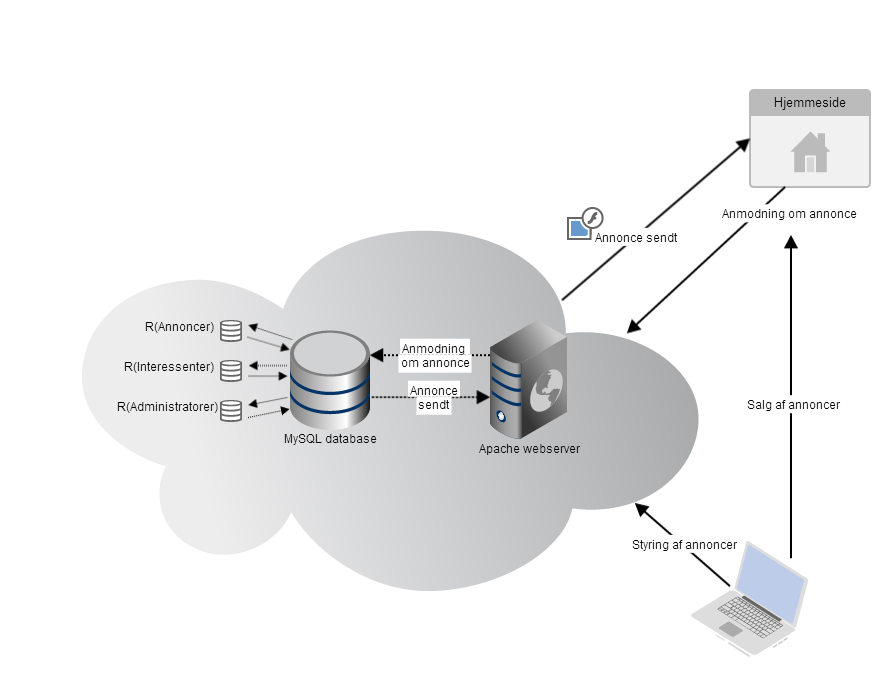
\includegraphics[width=\textwidth,height=\textheight,keepaspectratio]{architecture_diagram.png}

\section{Projektaftalen}

Projektet vil løbe over de kommende tre måneder. Projektet er en prototype og vil muligvis ikke være færdigt udviklet når perioden udløber. Projektet vil have til formål at udvikle et system det består af et interface og en database.  Interfacet skal være funktionelt og det skal være nemt at registrere annoncebannere. Det skal være muligt at registrere med hvilken vægtning et banner skal vises, samt registere en udløbsdato og/eller et maksimalt antal visninger for det pågældende banner. Derudover må et banner ikke vises på den samme hjemmeside mere end en gang.
Treuer Media's ejer Jan har indvilliget i at stå til rådighed ved aftestning af systemet. Derudover vil der være løbende kontakt med en ekstern person der kan svare på eventuelle spørgsmål.   

\section{Intern projektetablering}

Projektet er et open source bannerreklamesystem. Systemet skal kunne downloades og bruges af mindre ikke-kommercialle foreninger og interesseorganisationer, som ikke har de fornødne midler til at købe dyre systemer. Der findes på nuværende tidspunkt ikke noget nemt håndterligt open source bannerreklamesystem, så projektet skal være en nyudvikling, der er ment til at erstatte de nuværende brugte systemer. Projektet skal udvikles til et firma ved navn Treu Media. Treu Media er specialiceret indenfor annoncesalg og en lang række andre medieudgivelser. 
\newline
\newline
Projektgruppen er blevet informeret om at systemet har følgende betingelser. Det skal kunne bruges i alle browser. Systemet skal gøre det nemt at registrere bannnere. Det skal være muligt at angive med hvilken vægtning et banner skal vises. Systemet skal også gøre det muligt at registret en udløbsdato og/eller et maksimalt antal visninger for det pågældende banner. Derudover må det samme banner ikke vises flere gange på samme hjemmeside. 
Projektet har meget få betingelser og der er mange muligheder for udvidelse af projektet. Projektgruppen har stor mulighed for at påvirke projektet, og kommme med nye ideer til og udvidelser af projektet.
Projektgruppen har derfor valgt at sætte følgende begrænsning på systemet. Systemet er i første omgang kun ment til at blive brugt af Treu Medias ejer Jan. Jan er som udgangspunkt den eneste interessent.
\newline
\newline
Projektgruppen har endnu ikke haft et møde med Jan, men med en anden kontakt. Det er meningen at Jan kun vil være tilrådighed ved aftestning af systemet, eller hvis det opstår spørgsmål som kontaktpersonen ikke kan svare på. 
\newline
\newline
Yderligere har projektet til formål at styrke projektgruppens erfaringer indenfor web-udwikling og databaser.
Projektgruppen er opdelt således at Signar har det overordnede overblik over projektdelene. Han står derudover med ansvar for Javascript delen, da han har tidligere erfaring med dette. Aslak og Amanda fokusere på at styrke deres evner indenfor html, php og css, herunder bootstrap. Projektgruppen vil i fællesskab udvikle databasedelen.
\newline
\newline
Projektgruppen har valgt at bruge versionsstyringssystemet github. 
Projektet kan findes under følgender URL: https://github.com/AslakNiclasen/ProjektOpgave. Projektgruppen har derudover valgt at mødes hver torsdag evt. mandag om nødvendigt, gruppemøderne vil finde sted på DIKU. 
\newline
\newline 
\section{FACTOR-kriteriet}

\large{\bf{F}}\normalsize{unctionality
\\
- Visning af bannere med forskellig vægtning}
\newline
\newline
\large{\bf{A}}\normalsize{pplication domain
\\
- afhængigt af senariet er det enten Jan eller en it ansvarlig hos en organisation eller forening}
\newline
\newline
\large{\bf{C}}\normalsize{onditions\\
- Skal kunne bruges på tværs af browsere\\
- Skjult for brugere af hjemmesider\\
- Open source}
\newline
\newline
\large{\bf{T}}\normalsize{echnology\\
- Web-teknologi: html, css, php, javascript.\\
- Databaser}
\newline
\newline
\large{\bf{O}}\normalsize{bjects\\
- Bannere}
\newline
\newline
\large{\bf{R}}\normalsize{esponsibility\\
- Visning af bannere
- Holder styr på banner visning}

\newpage
\section{Bilag 1}
\begin{center}
\huge{\bf{Referat}}
\\
\normalsize{Projektgruppemøde}
\end{center}
Dato: 20/3-14
\newline
\newline
Tid: 11.30
\newline
\newline
Sted: Biocenteret
\newline
\newline
Inkaldte: Aslak, Signar og Amanda Bergqvist
\newline
\newline
Afbud: Ingen
\newline
\newline
\newline
\newline
Dagsorden:
\newline
\newline
1: Afklare spørgsmål vedrørende delrapport 1 og projektet.
\newline
\newline
2: Udele arbejdsopgaver i forhold til delrapport 1.
\newline
\newline
3: Aftale tidspunkt og dagsorden for næste møde.
\newline
\newline
\newline
\newline
Ad punkt 1:
Arbejdsfrekvens: Projektgruppen har aftalt at mødes hver torsdag, og mandag eller weekender om nødvendigt. 
\newline
\newline
Spørgsmål til instruktor: Literaturliste? fodnoter?
\newline
\newline
Ad punkt 2: Projektgruppen har aftalt at arbejde selvstændig på spørgsmålene indtil lørdag. På lørdag diskuteres spørgsmålene yderligere. Projektgruppen har aftalt at spørgsmålene skal være skrevet helt færdig til onsdag eftermiddag. 
Spørgsmålene er udeligeret som følger:   
\newline
\newline
(a) Signar 
\newline
\newline
(b) Aslak
\newline
\newline
(c) Signar 
\newline
\newline
(d) Aslak/ Amanda
\newline
\newline
(e) Amanda
\newline
\newline
FACTOR-kriteriet: Aslak
\newline
\newline
Referat: Amanda
\newline
\newline
Ad punkt 3: Projektgruppen har aftalt at næste møde er på DIKU på lørdag d. 22/3 kl 12. 
\newline
\newline
\newline
\newline
Referent: Amanda Bergqvist
\end{document}